\documentclass[12pt]{article}
\usepackage[a4paper, total={5.7in, 9in}]{geometry}
\usepackage{graphicx}
\usepackage{amsmath}
\usepackage{booktabs}
\usepackage{hyperref}
\usepackage{listings}
\usepackage{xcolor} 

\definecolor{sfondo}{HTML}{F8F8F8}      
\definecolor{numeri}{HTML}{888888}      
\definecolor{bordo}{HTML}{DDDDDD}      


\lstdefinestyle{stile}{
    backgroundcolor=\color{sfondo},     % Colore di sfondo
    basicstyle=\ttfamily\small,         % Font monospazio piccolo
    breaklines=true,                    % A capo automatico
    numbers=left,                       % Numeri di riga a sinistra
    numberstyle=\tiny\color{numeri},    % Stile dei numeri
    numbersep=10pt,                     
    frame=single,                       
    rulecolor=\color{bordo},            
    keepspaces=true,
    showspaces=false,
    showstringspaces=false,
}

% Diciamo a listings di usare questo stile come predefinito
\lstset{style=stile}


\begin{document}
\title{A Cognitive and Emotional Multi-Agent System\\ for Ludo Game Simulation}
\author{Kevin Nettikadan\\
{\em nettikadankevin@yahoo.com}}
\maketitle             

\section{Details of the proposal}
\label{sec:yourProposal}
The project consists of the design and implementation of a Multi-Agent System (MAS) to simulate a complete game of Ludo.
The primary goal is to model different cognitive and emotional player profiles using a BDI (Belief-Desire-Intention) architecture, leveraging VEsNA Pro frameworks to govern agent decision-making based on static temperaments and dynamic moods.
\subsection{Full specification of your proposal}
\label{subsec:specification}
The following section presents the original description submitted in the initial proposal form. This served as the conceptual foundation for the project, though the system was significantly expanded and refactored during the actual development phase to better reflect real-world dynamics.

\begin{quote}
\textit{I will implement a Multi-Agent System playing the board game "Ludo" using the VEsNA pro framework, as suggested by the professor. The game involves 4 players, each controlling 4 tokens. The goal is to race all tokens from a starting base to a central home area based on the roll of a dice. A crucial mechanic is interaction: landing on a square occupied by an opponent's token "eats" it, sending it back to the start. I will implement 4 Agents representing the players. These agents must perceive the board state and autonomously decide which token to move when multiple options are available. The 4 agents have different personality features to create distinct strategies (e.g., an "Aggressive" profile that prioritizes capturing opponents versus a "Prudent" profile that prioritizes safety).}
\end{quote}


\noindent The system evaluates how different predefined personalities interact within a competitive, multi-player environment with a single winner. The project integrates logical reasoning (Jason), environment management (CArtAgO), and emotional evaluation (VEsNA Pro). The finalized system is composed of:
\begin{itemize}
    \item A Ludo game environment that manages the objective game state, strict rules, and player interactions.
    \item Multiple agent profiles: 3 Static Cognitive Agents (Aggressive, Prudent, Balanced) and 1 Dynamic Emotional Agent (Emotive).
    \item A decision-making framework allowing agents to adapt strategies based on their current mood and temperament.
    \item A custom user interface for observing the game progress and agent behaviors.
\end{itemize}


\noindent During the implementation, several architectural improvements and functional expansions were introduced compared to the initial plan:
\begin{itemize}
    \item \textbf{Dummy Server:} Since the VEsNA framework was originally designed for embodied agents in 3D virtual environments (Godot engine), a lightweight Python WebSocket server was implemented to act as a dummy body endpoint, allowing the four agents to establish their required WebSocket connections without the need for a graphical 3D environment.
    \item \textbf{Enhanced Graphical Feedback:} Introduction of a multi-segment directional arrow system within the custom Java Swing GUI to visually trace agent decisions and trajectories before they are finalized on the board.
    \item \textbf{Concurrency and Pause State:} Implementation of a thread-safe Pause mechanism allowing the user to freeze the CArtAgO artifact and inspect Jason reasoning logs in real-time without causing deadlocks between the system and the interface.
\end{itemize}

\subsection{The kind of your proposal}
\label{subsec:kind}
This is a creative project classified as hard. It requires integrating the VEsNA
Pro emotional engine with standard BDI logic, mapping discrete board positions to
complex tactical evaluations (e.g., computing circular modular distances to hunt
opponents without overshooting), and carefully calibrating VEsNA temper arrays to
ensure distinct and recognizable behaviors across all four agents.


\pagebreak

\section{Domain Model}
\label{sec:intro}
\noindent This section describes the system's domain model, defining the rules, the physical entities, and the spatial logic of the simulated Ludo environment.

\subsection{The Ludo Board and Game Rules}
\label{subsec:board_rules}
\noindent Ludo is a classic board game for 2 to 4 players derived from the ancient Indian game Pachisi. 
It was chosen as the simulation environment because its
mechanics naturally produce the kinds of multi-agent interaction-cooperation,
competition, risk management, and emotional reactions, that the VEsNA Pro
framework is designed to model.


\noindent In this simulated environment, the game involves exactly 4 players (represented by our autonomous BDI agents), each controlling 4 tokens. All tokens begin the game off the board in a
dedicated starting area called the \textbf{Base}.
\linebreak

\noindent The turn structure is strictly sequential. On each turn, the active agent
rolls a single six-sided dice (values 1 to 6). A token may only leave the Base and
enter the shared outer track upon rolling a \textbf{6}, which represents the
exclusive condition for deployment. Once in play, tokens advance clockwise around
the outer perimeter by exactly the number of steps shown on the dice.

\noindent A crucial interaction mechanic governs the shared perimeter: if an
agent's token lands on a square already occupied by an opponent's token, the
opponent's token is \textbf{captured} (colloquially referred to as being
``eaten'') and immediately returned to its Base, where it must wait for another
roll of 6 to re-enter the game. This mechanic is the primary driver of conflict
and emotional reaction within the simulation.

\noindent While the shared outer track exposes tokens to these attacks, each
player has a private colored \textbf{safe zone} of 6 squares leading toward the
central area, accessible only to tokens of that specific color. Tokens navigating
this safe zone are completely immune to capture. The first agent to successfully
move all 4 tokens into the central \textbf{Home} area wins the simulation.


\begin{figure}[htbp]
    \centering
    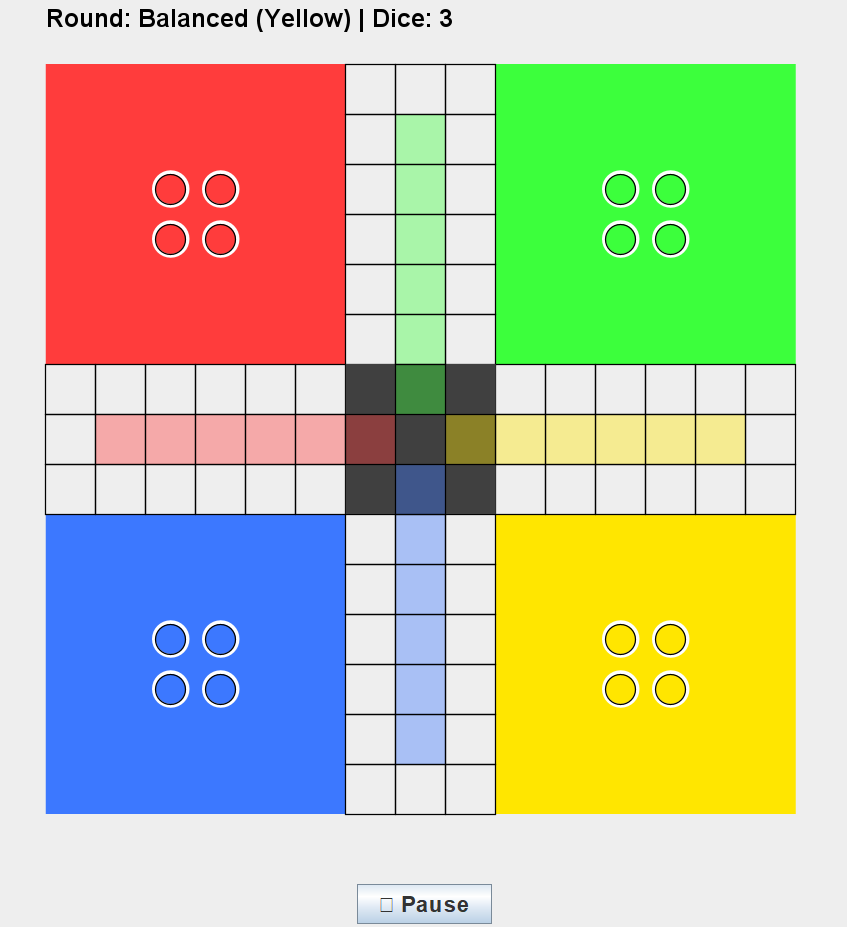
\includegraphics[width=0.75\textwidth]{Ludo_board_img.png}
    \caption{Initial board configuration in the Java Swing GUI. All 16 tokens 
are in their colored Base areas (corners). The shared white perimeter 
(52 squares), the four colored safe-zone corridors, and the central dark 
Home area are clearly visible. The GUI also displays the current player and the last dice roll in the status bar at the top.}
    \label{fig:ludo_board}
\end{figure}
\pagebreak  
\subsection{The Board and Spatial Logic}
\label{subsec:intro-level1}
\noindent To easily manage  the board state without hardcoding every single path for each player, the main perimeter of the Ludo board is mathematically modeled as a  \textbf{cyclical array of 52 absolute squares}. Each player's journey
starts at a fixed offset within this array. Since 4 players are equidistant on a
52-square board, their starting positions are separated by exactly 13 squares
each.

\noindent To calculate overlaps and potential attacks across this shared cyclical structure, agents use modular arithmetic. The absolute position on the shared board is calculated using the following formula:
\[ AbsPos = (PlayerID \times 13 + LogicalPos) \pmod{52} \]
\noindent where \texttt{PlayerID} ranges from 0 to 3 and \texttt{LogicalPos}
represents the token's position relative to its own starting point. This
mathematical abstraction allows any agent to compare its absolute position against
any opponent's absolute position, predicting collisions regardless of their
distinct starting points on the physical board.

\noindent Beyond the shared perimeter, each player has a private
\textbf{safe zone} consisting of 6 squares (logical indexes 51 to 56) that leads
to the final \textbf{Home} square (index 57). Tokens in this zone are only
accessible to the owning player and are immune to any form of capture.

\subsection{Token States}
\label{subsec:tokens}
\noindent Each agent controls 4 tokens. To simplify the BDI reasoning process, a token can exist in one of four distinct macro-states during the simulation, tracked by an integer representing its logical position:
\begin{itemize}
    \item \textbf{Base (-1):} The token is off the board. It requires a specific triggering event (a dice roll of exactly 6) to be deployed into the active arena at position 0.
    \item \textbf{In Play (0 to 50):} The token is navigating the outer shared perimeter. In this state, it is exposed to attacks and can itself attack opponents landing on the same absolute square.
    \item \textbf{Safe Zone (51 to 56):} The token has entered the final straight. It is completely invulnerable to attacks and is heading toward the winning condition.
     \item \textbf{Home (57):} The token has reached the central winning area. It no longer participates in the game. An agent wins when all 4 of its tokens reach this state.
\end{itemize}

\pagebreak
\section{Agents and Artifacts}
\label{sec:agents}
This section details the roles, psychological profiles and programmed behaviors of the specific components designed for the simulation.  The system
consists of one shared CArtAgO Artifact and four distinct Jason/VEsNA Pro agents.


\subsection{LudoBoard Artifact}
\label{subsec:artifact}
\noindent The \texttt{LudoBoard} Artifact, developed in Java using the CArtAgO framework, acts as the shared physical environment and the absolute source of
truth for the game state. It is responsible for:
\begin{itemize}
    \item  Maintaining \texttt{positions[4][4]}, tracking the logical position of
    all 16 tokens (4 agents $\times$ 4 tokens).
    \item Generating dice rolls via the \texttt{@OPERATION rollDice()} method.
    \item Resolving spatial conflicts by detecting overlaps using the absolute
    position formula and sending captured tokens back to Base.
    \item Exposing \textbf{observable properties} \texttt{current\_player},
    \texttt{dice}, \texttt{board\_state}, and individual properties of \texttt{token(P, T, Pos)},
    that the Jason agents continuously monitor to trigger their
    BDI reasoning cycles.
    \item Rendering the Java Swing GUI and managing concurrent access between the
    JaCaMo execution thread and the Swing Event Dispatch Thread (EDT).
\end{itemize}


\noindent The system follows the standard JaCaMo three-layer architecture: the
\textbf{Jason BDI engine} governs agent reasoning in \texttt{.asl} files, the
\textbf{CArtAgO framework} manages the shared \texttt{LudoBoard} artifact, and
\textbf{VEsNA Pro} adds the temperament-based plan selection layer on top of
standard Jason deliberation. Agents perceive the board exclusively through
CArtAgO observable properties and act on it through artifact operations
(\texttt{rollDice}, \texttt{moveToken}), never communicating directly with
each other.

\subsection{Temper Configuration Overview}
\label{subsec:temper_overview}
\noindent Each agent is assigned a \texttt{temper} vector in the \texttt{.jcm}
configuration file. This vector defines the agent's psychological baseline across
three static personality dimensions (\texttt{aggression}, \texttt{safety},
\texttt{advance}) and, for the fourth agent, two additional dynamic mood
dimensions declared with the \texttt{[mood]} tag. Table~\ref{tab:temper} provides
a comparative overview.

\begin{table}[htbp]
\centering
\begin{tabular}{|l|c|c|c|c|c|}
\hline
\textbf{Agent} & \textbf{aggression} & \textbf{safety} & \textbf{advance}
               & \textbf{anger} & \textbf{joy} \\
\hline
Aggressive (Red)  & 0.9 & 0.1 & 0.5 & ---                     & ---                     \\
Prudent (Green)   & 0.1 & 0.9 & 0.5 & ---                     & ---                     \\
Balanced (Yellow) & 0.5 & 0.5 & 0.7 & ---                     & ---                     \\
Emotive (Blue) & 0.5 & 0.5 & 0.5 & 0.1\textsuperscript{*}  & 0.8\textsuperscript{*}  \\
\hline
\end{tabular}
\caption{VEsNA Pro temper configuration for each agent. Values marked with
\textsuperscript{*} are mutable mood propensities (\texttt{[mood]}) that are
altered at runtime through plan \texttt{effects}.}
\label{tab:temper}
\end{table}

\noindent The Emotive agent adopts a neutral static baseline (\texttt{0.5}, \texttt{0.5}, \texttt{0.5})
equidistant from all personality extremes. The behavioral difference emerges exclusively from the dynamic
\texttt{anger}/\texttt{joy} dimensions, which shift at runtime in response to
game events.


\subsection{Aggressive Agent (Red)}
\label{subsec:agent_aggressive}
\noindent This agent represents a predatory playstyle. Its VEsNA \texttt{temper}
strongly prioritizes \texttt{aggression} ($0.9$) while minimizing \texttt{safety}
($0.1$). Its plan hierarchy is:

\begin{enumerate}
    \item \textbf{Eat an opponent} (\texttt{@eat\_enemy}, aggression $= 1.0$):
    If any token can land on an occupied square, this plan is the highest priority.
    \item \textbf{Deploy a new token} (\texttt{@exit\_base}, aggression $= 0.8$):
    On a roll of 6, the agent expands its presence on the board aggressively.
    \item \textbf{Hunt the nearest prey} (\texttt{@hunt\_prey}, aggression $= 0.6$):
    The agent seeks to capture the closest opponent. Using Jason's \texttt{.findall} and \texttt{.min}
    internal actions, the agent computes the \textbf{circular modular distance}
    to every enemy token after each possible move. It selects the token that
    positions itself closest behind a target without overshooting, maximising
    the chance of a capture on the following turn.
    \item \textbf{Enter safe zone} (\texttt{@advance\_safe}): A purely
    opportunistic retreat, applied only when the move enters into the protected
    corridor.
    \item \textbf{Fallback}: Passes the turn if no valid move exists.
\end{enumerate}

\subsection{Prudent Agent (Green)}
\label{subsec:agent_prudent}
\noindent The Prudent agent is highly risk-averse. Its VEsNA priorities are
mapped heavily toward the \texttt{safety} dimension ($0.9$). Its decision
hierarchy strictly favors:

\begin{enumerate}
    \item \textbf{Enter the safe zone} (\texttt{@reach\_safety}, safety $= 1.0$):
    The highest-priority plan. If any token is able to reach the private corridor in a
    single move, the agent will always take it.
    \item \textbf{Advance an exposed token} (\texttt{@advance\_token},
    safety $= 0.8$): Moving a token that is already on the shared perimeter is
    preferred over deploying new ones, as it reduces the number of exposed targets.
    \item \textbf{Deploy a new token} (\texttt{@exit\_base}, safety $= 0.2$):
    The lowest priority. The agent only deploys a new token when it rolls a 6
    and has no other legal action available.
    \item \textbf{Fallback}: Passes the turn.
\end{enumerate}

\subsection{Balanced Agent (Yellow)}
\label{subsec:agent_balanced}
\noindent The Balanced agent simulates rational human play by dynamically
evaluating the board state before committing to a strategy. Its key innovation
is the \textbf{army strategy}: using Jason's internal \texttt{.count()} function,
it evaluates how many of its tokens are currently active on the shared perimeter
(\texttt{active\_tokens}). Its plan hierarchy is:

\begin{enumerate}
    \item \textbf{Eat an opponent} (\texttt{@eat\_enemy}, aggression $= 0.7$):
    Opportunistic captures are taken but with less urgency than the Aggressive agent.
    \item \textbf{Enter the safe zone} (\texttt{@reach\_safety}, safety $= 0.8$):
    Protecting a token by moving it into the corridor is a high priority.
    \item \textbf{Deploy urgently} (\texttt{@exit\_base\_urgent}): If less than
    2 tokens are in play, a roll of 6 is immediately used to deploy. This plan has
    a temper perfectly matching the agent's baseline ($0.5, 0.5, 0.5$), giving it
    the highest possible similarity score in this scenario.
    \item \textbf{Advance} (\texttt{@advance\_token}): Standard progression
    once the army is sufficiently deployed.
    \item \textbf{Fallback}: Passes the turn.
\end{enumerate}

\subsection{Emotive Agent (Blue)}
\label{subsec:agent_emotive}
\noindent The Emotive agent is the experimental subject for the VEsNA Pro dynamic
mood engine. Its neutral static baseline ($0.5, 0.5, 0.5$) means that behavioral
direction is driven almost entirely by the mutable \texttt{anger}/\texttt{joy}
mood values.

\noindent \textbf{Calm state:} Initial mood (\texttt{anger = 0.1},
\texttt{joy = 0.8}) steers VEsNA Pro toward plans annotated with low anger and
high joy: cautious advancement and calm deployment.

\noindent \textbf{Trauma trigger:} The agent maintains a working memory using the
belief \texttt{in\_play(T)}, added when a token moves onto the board. If
\texttt{token(Me, T, -1)} fires and \texttt{in\_play(T)} is true, the agent
infers a capture event and triggers \\ \texttt{!react\_to\_death(T)}. The
\texttt{@got\_eaten} plan raises \texttt{anger} significantly via VEsNA Pro
\texttt{effects}.

\noindent \textbf{Angry state:} With high \texttt{anger}, the similarity
calculation strongly favors plans annotated with \texttt{anger(0.9)}, steering
the agent toward aggressive deployment and pursuit.

\noindent \textbf{Catharsis:} The agent returns to a calmer behavioral state when it successfully captures an opponent via a specific retaliatory plan (\texttt{@vendetta}). The execution of this plan directly alters the mood variables, reducing \texttt{anger} and restoring \texttt{joy}, allowing the emotional loop to close. The technical implementation of this transition, including the specific code and VEsNA Pro \texttt{effects}, is detailed in Section \ref{subsec:code_agents}.

\pagebreak

\section{System Architecture and Workflow}
\label{sec:architecture}
\noindent The overall architecture bridges objective physical events (managed by
the Java CArtAgO environment) with subjective agent reasoning (managed by the
Jason/VEsNA Pro BDI engine). Figure~\ref{fig:workflow} illustrates the complete
lifecycle of a single turn, which operates as a continuous feedback loop.

\begin{figure}[htbp]
    \centering
    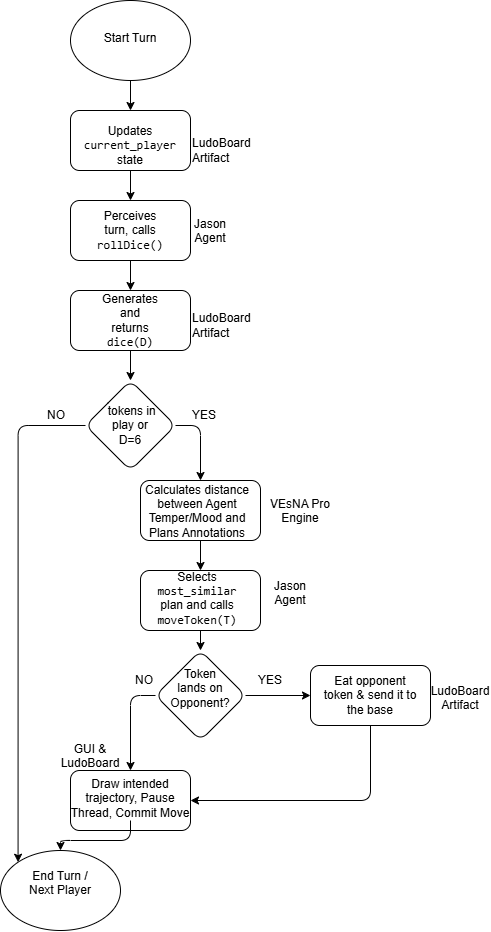
\includegraphics[width=0.55\textwidth]{S.drawio.png}
    \caption{Complete execution flow of a single turn. The diagram illustrates
    the interaction between the CArtAgO \texttt{LudoBoard} Artifact, the Jason BDI reasoning cycle, and the VEsNA Pro emotional
    plan selection engine.}
    \label{fig:workflow}
\end{figure}


\subsection{Turn Initialization and Perception}
\label{subsec:turn_init}
\noindent Each turn begins when the \texttt{LudoBoard} Artifact updates the
\texttt{current\_player} observable property. The corresponding Jason agent
perceives this change through CArtAgO's event notification mechanism and reacts
by triggering its \\ \texttt{+current\_player(Id)} plan, which invokes the
\texttt{rollDice()} artifact operation. The Artifact generates a random integer
from 1 to 6 and propagates it as an update to the \texttt{dice} observable
property, formally initiating the decision-making phase.

\subsection{Legal Move Filtering and BDI Deliberation}
\label{subsec:bdi_eval}
\noindent Upon perceiving the dice value \texttt{D}, the agent enters the BDI
deliberation cycle. First, \textbf{Jason evaluates the context conditions} of
all plans annotated for \texttt{!choose\_move(D)}. Only plans whose logical
guard is provable from the current belief base are admitted as \textbf{applicable
options}. For example:

\begin{itemize}
    \item \texttt{@eat\_enemy} is applicable only if \texttt{can\_eat(Me, T, P, D)}
    holds i.e., some token can land on an occupied enemy square.
    \item \texttt{@exit\_base} is applicable only if \texttt{D == 6} and at
    least one token is in the Base.
    \item \texttt{@advance\_token} is applicable only if a token is in play and
    the move does not exceed position 57.
\end{itemize}

\noindent If the agent has no tokens in play and the dice result is not 6, no
legal plan context is satisfied. The \textbf{fallback plan} (\texttt{@fallback\_move},
with a zero-vector temper) is activated, calling \texttt{moveToken(0, \_)} with no
real effect, and the turn passes immediately to the next player.

\noindent Once the applicable plan set is determined, the \textbf{VEsNA Pro engine}
evaluates the \texttt{temper} annotation of each applicable plan against the
agent's current full temper vector (including any live mood values for the Emotive
agent). Using the \texttt{most\_similar} strategy, the framework computes a
vectorial similarity score and probabilistically selects the plan whose emotional
and cognitive profile most closely matches the agent's current psychological state.

\subsection{Action Execution and Artifact Synchronization}
\label{subsec:action_exec}
\noindent The selected plan executes the \texttt{moveToken(T, \_)} CArtAgO
operation. The Artifact intercepts this call and applies the full movement logic:
it computes the new logical position, checks for spatial conflicts via
modular arithmetic, and if an opponent is captured, updates the opponent's token
position to $-1$ and fires the corresponding \texttt{token(P, T, -1)} observable
property update\textbf{, and finally} commits the final board state.


\section{User Interface}
\label{sec:ui}
\noindent The simulation features a custom Java Swing Graphical User Interface
(GUI) integrated directly with the underlying CArtAgO Artifact. This interface
serves both as a real-time game viewer and as an active \textbf{debugging and
observation tool} for the multi-agent system.

\subsection{Real-Time Playfield}
\label{subsec:playfield}
\noindent The GUI renders a traditional cross-shaped Ludo board using Java2D
graphics within a \texttt{BoardPanel} inner class that overrides
\texttt{paintComponent(Graphics g)}. Token coordinates are \textbf{mathematically
derived} from their logical positions on the cyclical array using the same formula
employed by the agents, ensuring pixel-perfect consistency between the internal
model and the visual output.

\noindent The board layout uses a 15$\times$15 grid of cells, each 40 pixels
wide, with the four colored corner areas representing the Base zones, the shared
white perimeter encoding the 52 cyclical squares, and the four colored corridors
representing the private safe zones. Tokens are rendered as filled circles with a
black outline, color-coded to their respective agent personality:

\begin{itemize}
    \item \textbf{Red} - Aggressive Agent
    \item \textbf{Green} - Prudent Agent
    \item \textbf{Yellow} - Balanced Agent
    \item \textbf{Blue} - Emotive Agent
\end{itemize}

\noindent A persistent \textbf{status bar} at the top of the panel displays the
currently active agent's name and the result of the last dice roll, providing
continuous contextual information to the observer.

\subsection{Visual Trajectory System}
\label{subsec:trajectory}
\noindent A challenge in MAS simulation is exposing the internal BDI
reasoning visually. To address this, a \textbf{multi-segment directional arrow
system} was implemented. Before an agent finalizes a \texttt{moveToken} action,
the GUI draws an arrow explicitly tracing the \textit{exact path} the token will
traverse, cell by cell, through the intermediate squares of the cyclical array.

\noindent The arrow uses two rendering layers: a thick black outer
stroke for contrast and a thinner inner stroke in the token's color. A filled
arrowhead polygon is computed using \texttt{Math.atan2}, ensuring correct
directionality regardless of trajectory orientation. Special cases (exiting Base,
entering safe zone) are handled separately.


\begin{figure}[htbp]
    \centering
    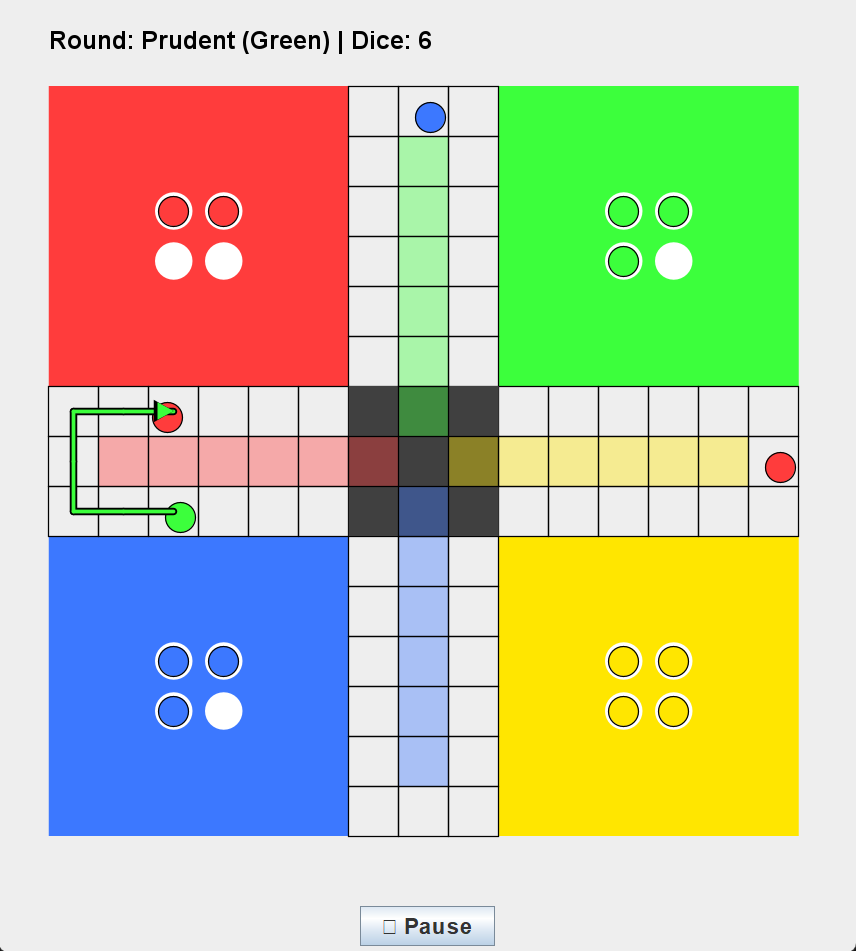
\includegraphics[width=0.9\textwidth]{freccia_ludo.png}
    \caption{The Java Swing GUI during an active game turn (Blue/Emotive agent,
    Dice: 3). The multi-segment directional arrow traces the planned trajectory
    of a token moving from the safe zone entry point.}
    \label{fig:gui}
\end{figure}

\subsection{Pause Mechanism and Thread Safety}
\label{subsec:pause}
\noindent A \textbf{Pause/Resume} toggle button is provided in a bottom control
panel. When activated, a \texttt{volatile boolean isPaused} flag is set to
\texttt{true}. The Artifact's \texttt{rollDice} and \texttt{moveToken} methods
each invoke \texttt{checkPause()} before any state change. This method enters a
low-frequency \textbf{polling loop} (\texttt{Thread.sleep(200ms)}), yielding CPU
time while awaiting resumption. This approach avoids the complexity of Java monitor
locks while guaranteeing no board state mutation during the pause window, preventing
deadlocks between the JaCaMo thread and the Swing EDT. 

\noindent This feature allows users to freeze the simulation precisely
during the trajectory visualization phase and cross-reference the visual move
with the agents' BDI logging outputs in the terminal, providing
real-time debugging capability.
%%%%%%%%%%%%%%%%    6   %%%%%%%%%%%%%%%%%%%%%%%%% 
\section{Code Specification and Implementation}
\label{sec:implementation}
\noindent This section details the technical stack used for the MAS and highlights the core architectural implementations that drive the simulation.

\subsection{Development Stack and Project Structure}
\label{subsec:stack}
\noindent The project is built upon the JaCaMo framework, combining three distinct technologies:
\begin{itemize}
    \item \textbf{Jason:} The AgentSpeak interpreter used for programming the BDI agents and defining their logical rules.
    \item \textbf{CArtAgO:} The framework utilized to build the \texttt{LudoBoard} environment in Java, bridging the gap between object-oriented logic and Jason perception.
    \item \textbf{VEsNA Pro:} Integrated directly to handle static personality traits (\texttt{temper}) and dynamic emotional states. The foundational VEsNA Pro framework and base code utilized in this project were provided by the course instructors \cite{vesna2024}.
\end{itemize}

\noindent The codebase follows the JaCaMo directory convention: The \texttt{src/env} directory contains the Java CArtAgO artifacts and GUI components, while the \texttt{src/agt} directory contains the \texttt{.asl} source files for the BDI agents. The entire system is orchestrated by the main \texttt{.jcm} configuration file.

\subsection{Spatial Collision Detection (\texttt{can\_eat})}
\label{subsec:can_eat}
 
\noindent The \texttt{can\_eat} rule is the mathematical core shared by the
Aggressive, Balanced, and Emotive agents. It determines whether a specific
token move would land on a square occupied by an enemy:
 

\begin{lstlisting}
can_eat(Me, T, P, D) :- 
    token(Me, T, P) & P >= 0 & (P + D) <= 50 & 
    token(Enemy, _, EnemyP) & Enemy \== Me & EnemyP >= 0 & EnemyP <= 50 & 
    ((Me * 13 + P + D) mod 52) == ((Enemy * 13 + EnemyP) mod 52).
\end{lstlisting}

 
\noindent The rule verifies three conditions simultaneously: the source token
is currently in play (\texttt{P >= 0}); the move stays within the shared
perimeter (\texttt{P + D =< 50}); and the destination's absolute position,
computed via the modulo formula, coincides with an enemy's absolute position.
This single rule replaces what would otherwise require iterating over every
possible board combination explicitly.

\subsection{Emotional Annotations and Vector Alignment}
\label{subsec:code_agents}
\noindent A critical design challenge in integrating VEsNA Pro was ensuring that the Cosine Similarity calculation prioritizes dynamic moods over static personality traits. To achieve this, the static traits (\texttt{aggression}, \texttt{safety}, \texttt{advance}) across all of the Emotive agent's plans were mathematically locked to a neutral baseline of \texttt{0.5}. By eliminating the variance in these three dimensions, the vector distance calculated by the engine is theoretically forced to depend entirely on the mutable \texttt{[mood]} values (\texttt{anger} and \texttt{joy}).

\noindent The intended transition from a calm state to a retaliatory state and the subsequent catharsis is structured through plan annotations. The following snippet illustrates the design of the \texttt{@vendetta} plan:

\begin{verbatim}
// Retaliatory action requiring high anger while maintaining the neutral baseline
@vendetta[
    temper([aggression(0.5), safety(0.5), advance(0.5), anger(0.9), joy(0.1)]),
    effects([anger(0.0), joy(1.0)]) 
]
+!choose_move(D) : my_id(Me) & can_eat(Me, T, P, D) <-
    .print(" Emotive Move (Catharsis): Token ", T, " captured an enemy!");
    moveToken(T, _).
\end{verbatim}

\noindent From an architectural standpoint, this strict alignment was designed to guarantee that when the agent experiences trauma, the \texttt{anger(0.9)} annotation would naturally dominate the similarity score, forcing the selection of retaliatory actions. Furthermore, the \texttt{effects} vector was explicitly configured to use absolute boundary values (\texttt{anger(0.0), joy(1.0)}) to ensure a clean mood reset upon successful retaliation. 

\noindent However, as detailed in Section \ref{subsec:emotional}, empirical testing revealed that while this vector alignment is mathematically sound, the actual execution of the emotional loop is hindered by framework-level limitations regarding mood state persistence.
\subsection{Environment and Concurrency Management}
\label{subsec:code_env}
\noindent The \texttt{LudoBoard.java} artifact acts as the absolute source of truth. As detailed extensively in Section \ref{subsec:pause}, the \texttt{moveToken} operation prevents race conditions between the JaCaMo reasoning cycle and the Java Swing EDT via a polling loop, successfully avoiding monitor lock complexities and ensuring thread safety.

\subsection{System Configuration (\texttt{.jcm})}
\label{subsec:jcm}
 
\noindent The \texttt{.jcm} file declares the full MAS, including agent classes,
temper values, WebSocket addresses, and initial goals. The Emotive agent's entry
demonstrates the \texttt{[mood]} tag syntax:
 

\begin{verbatim}
agent emotive : emotive_agent.asl {
    ag-class:  vesna.VesnaAgent
    temper:    temper( aggression(0.5), safety(0.5), advance(0.5),
                       anger(0.1)[mood], joy(0.8)[mood] )
    strategy:  most_similar
    address:   localhost
    port:      9083
    goals:     start
}
\end{verbatim}

 
\noindent The \texttt{[mood]} tag is critical: without it, VEsNA Pro treats
\texttt{anger} and \texttt{joy} as immutable personality traits and silently
ignores all \texttt{effects} at runtime, disabling the emotional feedback system
entirely.

\subsection{Execution Instructions}
\label{subsec:execution}
\noindent To run the simulation, ensure that a compatible Java Development Kit (JDK) and Python 3 are installed. The execution requires two sequential steps:

\begin{enumerate}
    \item \textbf{Start the Dummy Server:} Open a terminal, navigate to the server directory, and execute the Python WebSocket script to initialize the body endpoints for the agents:
\begin{verbatim}
python dummy_server.py
\end{verbatim}
    
    \item \textbf{Launch the MAS:} Once the Python server is actively listening, open a new terminal in the root project directory and use Gradle to build and run the multi-agent system:
\begin{verbatim}
gradle run
\end{verbatim}
\end{enumerate}

\noindent Upon successful execution, the Java Swing GUI will automatically initialize, the agents will establish their WebSocket connections to the dummy server, and the autonomous Ludo simulation will begin. The simulation can then be controlled via the Pause/Resume button in the interface.

\subsection{Use of Artificial Intelligence and LLMs}
\label{subsec:ai_usage}
\noindent LLMs and Generative AI were utilized as auxiliary tools during the development of this project for the following specific tasks:
\begin{itemize}
    \item \textbf{Code Generation and Setup:} To automate the writing of repetitive structural components and to assist in the initial setup of the project structure.
     \item \textbf{GUI syntax:} Providing guidance on Java Swing API usage and layout management.
    \item \textbf{Language and Documentation:} To perform grammatical, stylistic, and formatting checks throughout this academic report.
\end{itemize}




\section{Results and Observations}
\label{sec:results}
\noindent This section presents and analyses the behavioral patterns observed
across multiple simulation runs, drawing directly from system log outputs.
The goal is to verify whether the VEsNA Pro temper configuration produces
meaningfully distinct agent behaviors, and whether the emotional state machine
of the Emotive agent functions as designed.

\subsection{Observed Agent Behavioral Patterns}
\label{subsec:behaviors}
\noindent All four agents demonstrated recognizably distinct behavioral profiles
consistent with their configured \texttt{temper} vectors.

\paragraph{Aggressive Agent.}
\noindent The Aggressive agent's advanced hunting logic implemented via
\texttt{.findall} and \texttt{.min} on circular modular distances was
consistently active throughout observed games. The following log sequence is
representative:

\begin{lstlisting}
[aggressive] I rolled a 4. Looking for the best move...
[aggressive] Aggressive Move : Move the token 0 to get closer to the prey.
[aggressive] I rolled a 5. Looking for the best move...
[aggressive] Aggressive Move : Use 5 to EAT an enemy with token 0!
  EATEN P0 has eaten a token from P3
\end{lstlisting}

\noindent This sequence confirms that \texttt{@hunt\_prey} correctly positioned
the token at the optimal chasing distance, and the subsequent \texttt{@eat\_enemy}
plan was triggered on the following turn as intended. In one observed full game,
the Aggressive agent performed the most captures of any agent, validating the
effectiveness of its targeting algorithm.

\paragraph{Prudent Agent.}
\noindent The Prudent agent demonstrated a highly risk-averse, "one-at-a-time" strategy. Because the \texttt{@exit\_base} plan has the lowest priority (\texttt{safety = 0.2}), the agent strongly prefers advancing an already exposed token rather than deploying new ones. Once a token is in play, the agent consistently focuses all its dice rolls on moving that specific token toward the safe corridor:
\begin{lstlisting}
[prudent] I rolled a 6. Looking for the best move...
[prudent] Prudent Move: I move the token 0 to be safe from the enemies.
\end{lstlisting}

\noindent The agent acts to minimize its footprint on the shared perimeter, attempting to secure one token in the safe zone before bringing a new target onto the board. When the dice roll allows a token to step into the final private corridor, the agent reliably prioritizes that absolute safety over any other available action.

\paragraph{Balanced Agent.}
\noindent The Balanced agent's army strategy is the main concept. The
\texttt{active\_tokens} counter correctly triggered the urgent deployment plan
when the agent had fewer than 2 tokens in play:

\begin{lstlisting}
[balanced] I rolled a 6. Looking for the best move...
[balanced] Balanced Move (Army): I have only 0 tokens out! I use the 6 to deploy the token 3!
...
[balanced] I rolled a 6. Looking for the best move...
[balanced] Balanced Move (Army): I have only 1 tokens out! I use the 6 to deploy the token 2!
\end{lstlisting}

\noindent Once two tokens were active, the agent transitioned smoothly to the standard advancement strategy (\texttt{@advance\_token}),
 demonstrating good dynamic priority management.
 This continuous re-evaluation proved highly adaptive during gameplay: if opponents captured its tokens,
 the agent's internal active token count dropped accordingly.
 This immediately caused the agent to shift its priority back to urgent deployment upon its next roll of 6,
 automatically attempting to rebuild its presence on the board rather than stubbornly advancing a single surviving token.

\subsection{Attempted Emotional Transitions (Emotive Agent)}
\label{subsec:emotional}
\noindent The intended design for the Emotive agent was to create a closed feedback loop where a token capture triggers an angry retaliatory state, which is eventually resolved through catharsis. However, empirical observation of the simulation logs revealed a critical failure in the emotional state machine's execution. The following log excerpt captures the anomaly:
\pagebreak
\begin{lstlisting}
  EATEN P2 has eaten a token from P3
[emotive_player] Emotive Event: Token 0 was captured! Anger level spiked to maximum.
[emotive_player] I rolled a 1. Looking for the best move...
[emotive_player] I pass this turn because I have no valid moves.
...
[emotive_player] I rolled a 6. Looking for the best move...
[emotive_player] Emotive Move (Calm): Peacefully deploying token 0 from the base.
\end{lstlisting}

\noindent This sequence demonstrates a clear disconnect between the BDI logical layer and the VEsNA Pro emotional engine. The Jason interpreter correctly intercepts the capture event via the \texttt{in\_play(T)} working memory and successfully fires the internal trauma trigger (printing the spike in anger). However, the VEsNA Pro framework fails to persist the \texttt{effects([anger(1.0), joy(0.0)])} mutation across turn boundaries. 

\noindent When the agent is called to deliberate on its next valid move (e.g., upon rolling a 6), the internal mood vector has already reset to its initial state. The \texttt{most\_similar} strategy evaluates the applicable plans using the original calm baseline (\texttt{joy = 0.8}), completely ignoring the trauma. Consequently, the agent incorrectly selects the \texttt{@exit\_base\_calm} plan, rendering the "Angry" state and the subsequent "\texttt{@vendetta}" catharsis practically unreachable during live gameplay.


\subsection{Limitations}
\label{subsec:limitations}
\noindent Several limitations were identified during the evaluation phase:

\begin{itemize}
   \item \textbf{No Inter-Agent Communication:} Agents have no mechanism to
    share information or coordinate strategies. All reasoning is performed
    independently based on the shared observable properties of the artifact.
    This is a fundamental constraint of the current JaCaMo configuration and
    eliminates the possibility of coalition or deception strategies.

   \item \textbf{VEsNA Pro Mood State Persistence:} As highlighted in Section \ref{subsec:emotional}, a systemic limitation was observed within the VEsNA engine's state management.
   When \texttt{[mood]} \texttt{effects} are triggered dynamically by reactive sub-goals (such as intercepting a capture event outside the standard \texttt{!choose\_move} deliberation cycle), the framework fails to persist the updated mood vector for subsequent turns.
   This prevents the execution of complex emotional state machines, as the agent suffers from "emotional amnesia" between turns.
\end{itemize}

\section{Conclusions and Future Improvements}
\label{sec:conclusions}
\noindent This project demonstrates the design and implementation 
of a competitive Multi-Agent System that successfully models 
distinct tactical profiles through VEsNA Pro temper vectors, 
while exposing important limitations in the framework's emotional 
state persistence mechanisms.

\noindent The attempt to model dynamic emotional states (trauma, anger, and catharsis) via the VEsNA Pro framework provided valuable architectural insights. While the vector-based \texttt{temper} alignment was mathematically sound, the simulation exposed critical limitations in the framework's ability to persist emotional mutations (\texttt{effects}) across turn boundaries. This "emotional amnesia" highlights a crucial area for future development in affective computing frameworks: the need for robust state persistence when emotions are triggered asynchronously by environmental trauma rather than standard deliberate actions.

\subsection{Future Improvements}
\label{subsec:future_improvements}
\noindent While the current simulation effectively proves the viability of combining cognitive and emotional AI, future iterations of this project could significantly expand the emotional complexity of the agents:

\begin{itemize}
    \item \textbf{Full OCC Emotional Model:} The current implementation focuses primarily on Anger and Joy. Integrating the broader OCC (Ortony, Clore, Collins) emotional model would allow agents to experience a wider spectrum of states. For instance, an agent could compute "Fear" when a highly Aggressive opponent is spatially approaching from behind, or "Relief/Satisfaction" upon successfully moving a token into the absolute safety of the inner zone.
    \item \textbf{Human-in-the-Loop (Hybrid Mode):} The current environment is a closed-loop AI simulation. Introducing a hybrid mode that allows a human player to control one set of tokens against three VEsNA-driven AI profiles would be a highly valuable addition. This would provide empirical data on human-AI tactical interactions, allowing researchers to measure if human players can recognize, predict, or be manipulated by the emotional states of their virtual opponents.
\end{itemize}

\vspace{1cm}
\nocite{*}
\bibliographystyle{splncs04}
\bibliography{bibliography}


\end{document}